
\chapter{Local Methods}
\label{chapter:local_methods}
Local methods mean that any change in a control point does not necessarily
affects 
the {\em entire} parameterization.  This is generally very desirable, as
changes can be focused on a specific region, without
disrupting the balance of the parameterization.
However, local methods are more complicated than non-local methods, 
and require definition over intervals, as well be seen below.

\section{General Splines}
Let a collection of $n+1$ points $(x_i, y_i)$ for $ i=0, 1, \ldots, n$ 
approximate the function $y=f(x)$ over the domain $[x_0, x_n]$.  In total, 
there are $n+1$ points and $n$ intervals.  
Let $S(x)$ be the piecewise continuous spine that
threads through each of the points $(x_i, y_i)$.  
For $x \in [x_i, x_{i+1}]$ and  $i=0, 1, \ldots, n-1$, 
the spline takes on $n$ 
interval definitions as follows: 
\be
S_i(x) 
\defe a_i + b_i (x - x_i) + c_i (x - x_i)^2 
+ d_i (x - x_i)^3 + 
\cdots + z_i (x - x_i)^p. 
\ee
where constant coefficients\footnote{Here the $z_i$
is arbitrary, meant to denote the last coefficient, but not necessarily the 
twenty-sixth coefficient.}
multiply successive powers\footnote{The powers are non-negative integers.} 
of $(x-x_i$), summed
to an arbitrary polynomial power $p$.  This is referred to as the {\bf
interval spline definition} to polynomial degree $p$.
Below we consider linear splines ($p=1$), quadratic splines ($p=2$), and
cubic splines ($p=3$).

\section{Linear Splines}
For linear splines, the interval spline definition is
\be
S_i(x) 
\defe
a_i + b_i (x - x_i)
\;\;\;
\mbox{for}
\; x \in [x_i, x_{i+1}] \;\mbox{and}\; i=0, 1, \ldots, n-1.
\ee
For any collection of points $(x_i, y_i)$, all coefficients $a_i$ and
$b_i$ for $i=0, 1, \ldots, n-1$ can be found using the {\bf zeroth derivative
continuity constraint}, which creates a spline that connects to each point
at the beginning and end of each interval, thus
\be
S_i(x_i) = y_i 
\;\;\;
\mbox{and}
\;\;\; 
S_i(x_{i+1}) = y_{i+1}
\;\;\;\mbox{for}\;i=0, 1, \ldots, n-1.
\ee
Here we see there are two constraints per interval $i$ and two unknowns, 
$a_i$ and $b_i$, per interval $i$.  The unknowns can be found directly by
evaluating the interval spline definition with each of the two constraint
equations.  In turn, these are, for 
$i=0, 1, \ldots, n-1$,
\begin{align}
S_i(x_i) 
&
= a_i + b_i(x_i - x_i) 
\overset{\mbox{\footnotesize set}}{=} y_i 
\implies 
a_i = y_i, \;\mbox{and}
\\
S_i(x_{i+1}) 
& 
= a_i + b_i (x_{i+1} - x_i) 
\overset{\mbox{\footnotesize set}}{=} y_{i+1}
\implies
b_i = \frac{y_{i+1} - y_i}{x_{i+1} - x_i}.
\end{align}
No additional continuity constraints can be created since the linear
spline has only $C^0$ continuity, meaning no derivatives of the 
function $S_i(x)$ are continuous.

\begin{Hexpo}
{Let $y = f(x) = \sin(\pi x)$ for $x \in [0, 1]$ be approximated by a linear
spline and a collection of three points equally spaced on the domain.  
Note $n+1 = 3$, thus $n=2$, indicating three points and two intervals.
Table~\ref{tab:linear_spline_example} summarizes the spline data.
Figure~\ref{fig:linear_spline_example}(a) shows the $\sin$ function and the
linear spline interpolations.
\begin{table}[h]
\caption{Linear spline approximation of $y = f(x) = \sin(\pi x)$ 
using three points and two intervals.}
% \centering
\begin{center}
\begin{tabular}{c|c|ccc|ccc}
$i$ & $x_i$ & $y_i$ & $\implies$  & $a_i$ & $b_i$ & $\implies$ & $S_i(x)$
\\
\hline \hline
0 & 0/2 & 0 &  & 0 & 2 &   & $2 x$
\\
1 & 1/2 & 1 &  & 1 & -2 &   & $1 - 2(x - 1/2)$
\\
2 & 2/2 & 0 &  & --- & --- &   & ---
\end{tabular}
\end{center}
\label{tab:linear_spline_example}
\end{table}
} % end Hexpo
\end{Hexpo}

\newpage
\begin{Hexpo}
{Repeat the previous example, but now with a
collection of five points equally spaced on the domain.  
Thus $n+1 = 5$, thus $n=4$, indicating five points and four intervals.
Table~\ref{tab:linear_spline_example_two} summarizes the spline data.
Figure~\ref{fig:linear_spline_example}(b) shows the $\sin$ function and the
linear spline interpolations.
\begin{table}[h]
\caption{Linear spline approximation of $y = f(x) = \sin(\pi x)$ 
using five points and four intervals.}
% \centering
\begin{center}
\begin{tabular}{c|c|ccc|ccc}
$i$ & $x_i$ & $y_i$ & $\implies$  & $a_i$ & $b_i$ & $\implies$ & $S_i(x)$
\\
\hline \hline
0 & 0/4 & 0 &  & 0 & $2\sqrt{2}$ &   & $2\sqrt{2} x$
\\
1 & 1/4 & $\sqrt{2}/2$ &  & $\sqrt{2}/2$ & $4 - 2\sqrt{2}$ &   
& $\sqrt{2}/2 + (4-2\sqrt{2})(x - 1/4)$
\\
2 & 2/4 & 1 &  & 1 & $2\sqrt{2} - 4$ &   & $1 + (2\sqrt{2}-4)(x - 2/4)$
\\
3 & 3/4 & $\sqrt{2}/2$ &  & $\sqrt{2}/2$ & $-2\sqrt{2}$ &   & $\sqrt{2}/2 - 
2\sqrt{2}(x - 3/4)$
\\
4 & 4/4 & 0 &  & --- & --- &   & ---
\end{tabular}
\end{center}
\label{tab:linear_spline_example_two}
\end{table}
} % end Hexpo
\end{Hexpo}

% \clearpage
\begin{figure}[htb]
  \begin{center}
    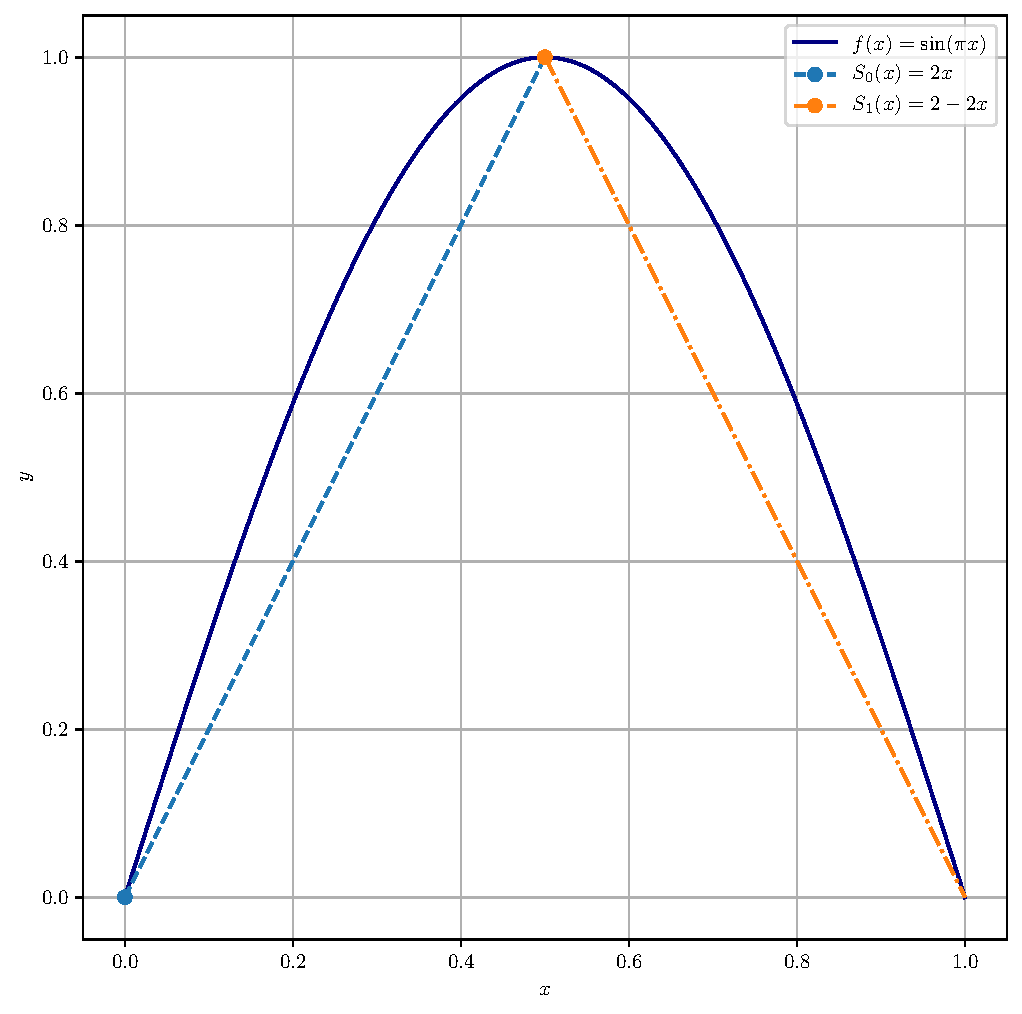
\includegraphics[width=\textwidth]{fig/linear_spline.pdf}
  \end{center}
    \caption{Linear spline example (a) with three points and (b) with five 
    points, see Table~\ref{tab:linear_spline_example_two} for individual 
    definitions of $S_i(x)$.
    Reference: fig/linear\_spline.py.}
  \label{fig:linear_spline_example} % label must come after caption 
\end{figure}


\clearpage
\section{Quadratic Splines}

For quadratic splines, the interval spline definition is 
\be
S_i(x) \defe a_i + b_i (x - x_i) + c_i (x - x_i)^2
\;\;\;
\mbox{for}
\; x \in [x_i, x_{i+1}] \;\mbox{and}\; i=0, 1, \ldots, n-1.
\ee


\section{Cubic Splines}
Cubic splines are useful because of their inherent smoothness.  
The cubic spline, its first derivative, and its second derivative are all
continuous.  Starting with the cubic spine's third derivative, discontinuity
arises.

Let a collection of $n+1$ points $(x_i, y_i)$ for $ i=0, 1, \ldots, n$ 
approximate the function $y=f(x)$ over the domain $[x_0, x_n]$.  In total, 
there are $n+1$ points and $n$ intervals.  
Let $S(x)$ be the piecewise continuous spine, cubic in this case, that
threads through each of the points $(x_i, y_i)$.  The spline takes on $n$ 
interval definitions as follows: 
\be
S_i(x) \defe a_i + b_i (x - x_i) + c_i (x - x_i)^2 + d_i (x - x_i)^3
\;\;\;
\mbox{for}
\; x \in [x_i, x_{i+1}] \;\mbox{and}\; i=0, 1, \ldots, n-1.
\ee
The $n$ foregoing definitions, with the coefficients $a_i, b_i, c_i, d_i$,
give rise to $4n$ (currently unknown) parameters 
used to define the complete spline $S(x)$.  Note that maintain its cubic nature, 
the spline must have $d_i \neq 0$.

Next we endow the spline with constraints on continuity and differentiability,
which allow the $4n$ unknown parameters to be solved.  First, function
continuity requires that the spline, on a particular interval, thread through
collection of points $(x_i, y_i)$ and the beginning and end of each interval.  
Thus, 
\be
S_i(x_i) = y_i \;\mbox{and}\; S_i(x_{i+1}) = y_{i+1}
\;\;\;\mbox{for}\;i=0, 1, \ldots, n-1.
\ee
This is the {\bf continuity constraint}, 
which gives rise to $2n$ conditions\footnote{Two conditions per interval
times $n$ intervals yields $2n$ conditions.}
and creates a spline that
is piecewise continuous.
Next, consider two {\bf differentiability constraints}, which state that the
first and second derivatives at a point $x_i$ are continuous.  That is, 
the first and second derivatives approaching a point $x_i$ from the interval
to the left side of the point must match the respective first and second 
derivatives
approaching the point $x_i$ from the interval to the right side of the point:
\be
S'_{i-1}(x_i) = S'_{i}(x_i) 
\;\mbox{and}\; 
S''_{i-1}(x_i) = S''_{i}(x_i) 
\;\;\;\mbox{for}\;i=1, 2, \ldots, n-1.
\ee
Because they apply only to the interior points
(and not the endpoints $x_0$ and $x_n$), the differentiability constraints
give rise to $2(n-1)$ constraints.\footnote{Two conditions per interior
point times $n-1$ interior points yields $2(n-1)$ conditions.}

Finally, two more conditions are necessary to completely define the spline
$S(x)$.  The two conditions are obtained by specifying differentiability
conditions on the two spline endpoints $x_0$ and $x_n$.  
Frequently, the first derivative is set to the known value of the function's
derivatives at the endpoints, 
\be
S'_0(x_0) = f'(x_0) 
\;\mbox{and}\; 
S'_{n-1}(x_n) = f'(x_n).
\ee
This is defined as a {\bf clamped spline}.
Alternatively, a {\bf natural spline} defines the second derivatives to be
zero at the endpoints, 
\be
S''_0(x_0) = 0 
\;\mbox{and}\; 
S''_{n-1}(x_n) = 0.
\ee
Finally, a {\bf not-a-knot} spline requires no additional constraints on the 
endpoint derivatives,\footnote{This has no effect on the original continuity
constraint on the endpoints, that $S_0(x_0) = y_0$ and $S_{n-1}(x_n) = y_n$.}
but requires that the {\em third} derivative be continuous at $x_1$ and 
$x_{n-1}$.

\section{B-Splines}
A {\bf B-spline} is a spline composed of two or more B\'ezier curves, joined 
end-to-end, subject to certain restrictions, which will be discussed below.
The ``B'' in B-spline stands for {\bf basis}, as the spline
curves, defined over an interval, utilize
control points that are interpolated with basis functions.
In contrast, 
general splines (\eg the linear, quadratic, and cubic 
splines discussed in the previous sections)
use data points that are interpolated directly, without basis functions.

B-splines are {\bf parametric}, so the functional form for a general
B-spline curve $\vS \in \realthree$, will will be written
explicitly as $\vS(t; \vx)$, similar to the notation introduced with
the B\'ezier curves in Section~\ref{sec:bezier_curves}.  Similar to
the B\'ezier 
compact notation discussed previously, B-spline 
curves are typically written in terms of the parametric variable $t$, without
the explicit notation of the space coordinates 
$\vx$ of the control points, \ie $\vP_i(\vx) = \langle \; x_i, y_i, z_i
\; \rangle$.

Similar to the definition of a general B\'ezier curve $\vC_p(t)$ of degree
$p$ in (\ref{eq:general_bezier_curve}), the general form for a 
B-spline $\vS_p(t)$ of degree $p$, with $n+1$ (not necessarily $p+1$, as
with B\'ezier curves) control points 
$\vP_i$, $i=0, 1, \ldots, n$, is given by
\be
\vS_p(t) \defe \sum_{i=0}^n N_{i,p}(t) \vP_i, 
\ee
where $N_{i,p}$ is the {\bf normalized basis function} and $\vP_i \in \realthree$
are the control points $\vP_0, \vP_1, \ldots, \vP_n$.
The normalized basis functions are defined by the {\bf Cox-de~Boor recursion
formulas}:
\be
\mbox{for } p=0: \;\;\; N_{i,0}(t) \;\; \defe \;\;
\left\{
\begin{tabular}{cl}
1
&
if $t_i \leq t < t_{i+1}$,
\\
0 
& 
otherwise.
\end{tabular}
\right.
\ee
%
\be
\mbox{for } p\geq 1: \;\;\; 
N_{i,p}(t) \;\; \defe \;\;
\dst\frac{\;\;\;\;t - t_i}{t_{i+p} - t_i} \; N_{i,p-1}(t) 
\;\; + \;\;
\dst\frac{t_{i+p+1} - t\;\;\;\;\;}{t_{i+p+1} - t_{i+1}} \; N_{i+1,p-1}(t).
\ee
The structure of the Cox-de~Boor recursion formulas is shown below through
illustrations of linear ($p=1$), quadratic ($p=2$), and cubic ($p=3$)
examples.
% make sure to break with LF prior to Hexpo
\\  % This is the break
%  
\begin{Hexpo}
{% Hexpo open
Linear B-spline ($p=1$): \\
\be
\mbox{for } p=1: \;\;\;
N_{i,1}(t) = 
\dst\frac{\;\;\;\;t - t_i}{t_{i+1} - t_i} \; N_{i,0}(t) 
\;\; + \;\;
\dst\frac{t_{i+2} - t\;\;\;\;\;}{t_{i+2} - t_{i+1}} \; N_{i+1,0}(t)
\ee
The linear forms are shown in the middle subfigure of Figure~\ref{fig:bspline}.
}% Hexpo close
\end{Hexpo}
\\
%
\begin{Hexpo}
{% Hexpo open
Quadratic B-spline ($p=2$): \\
\be
\mbox{for } p=2: \;\;\;
N_{i,2}(t) = 
\dst\frac{\;\;\;\;t - t_i}{t_{i+2} - t_i} \; N_{i,1}(t) 
\;\; + \;\;
\dst\frac{t_{i+3} - t\;\;\;\;\;}{t_{i+3} - t_{i+1}} \; N_{i+1,1}(t)
\ee
The linear forms are shown in the bottom subfigure of Figure~\ref{fig:bspline}.
}% Hexpo close
\end{Hexpo}
\\
%
\begin{Hexpo}
{% Hexpo open
Cubic B-spline ($p=3$): \\
\be
\mbox{for } p=3: \;\;\;
N_{i,3}(t) = 
\dst\frac{\;\;\;\;t - t_i}{t_{i+3} - t_i} \; N_{i,2}(t) 
\;\; + \;\;
\dst\frac{t_{i+4} - t\;\;\;\;\;}{t_{i+4} - t_{i+1}} \; N_{i+1,2}(t)
\ee
}% Hexpo close
\end{Hexpo}

\begin{figure}[h!]
  \begin{center}
    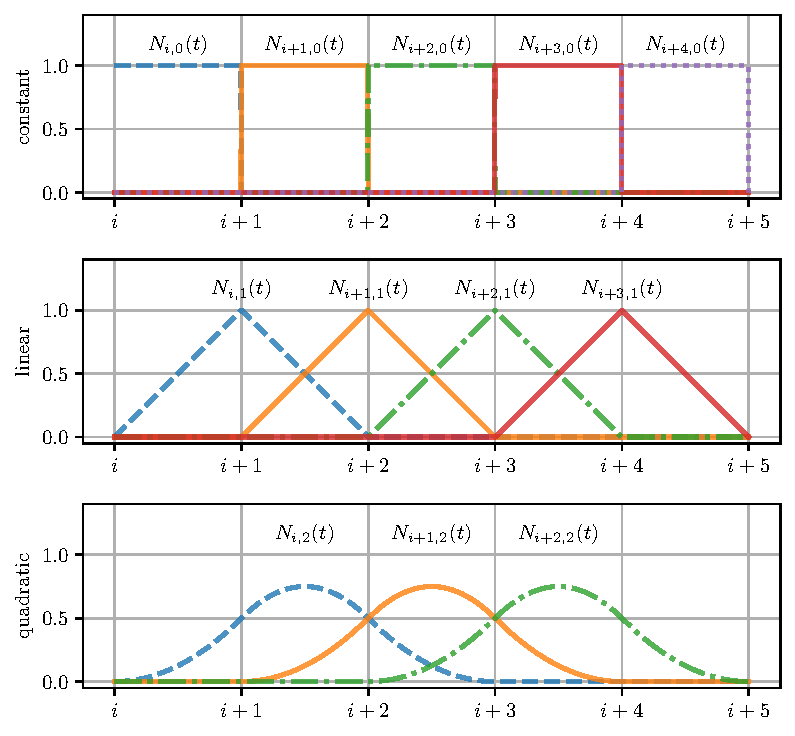
\includegraphics[width=\textwidth]{fig/bspline.pdf}
  \end{center}
    \caption{Normalized basis functions of the Cox-de Boor recursion formula
    for constant, linear, and quadratic forms.
    Reference: fig/bspline.py.}
  \label{fig:bspline} % label must come after caption 
\end{figure}

The discrete values (\eg
$t_i$, $t_{i+1}$, $t_{i+2}$, $t_{i+3}$, $t_{i+4}$, $t_{i+p}$, and $t_{i+p+1}$)
are referred to as {\bf knots}, which
mark the termination points, beginning or end, of an interval for the
parameter $t$.  The collection of all knots is called a {\bf knot vector}, 
designated by $\vT$.
We define the knot vector $\vT$
as a non-decreasing set of non-negative integer coordinates 
in parameter space, 
\be
\vT \defe 
\langle 
\; t_0, t_1, t_2, \ldots, t_m \;
\rangle.
\ee
The values for parameter $t$ are $t \in \real \subset [t_0, t_m]$
In total, there are $(m+1)$ knots in knot vector $\vT$.

\begin{Hexpo}
{% Hexpo open
A uniform knot vector containing 10 knots is written as
\be
\vT = \langle\; 0, 1, 2, 3, 4, 5, 6, 7, 8, 9 \; \rangle, \mbox{ with } 
t \in \real \subset [0, 9].
\ee
}% Hexpo close
\end{Hexpo}




To construct the B-spline $\vS_p(t)$ with normalized basis 
functions $N_{i,p}(t)$,
$(n+1)$ control points 
$\vP_0, \vP_1, \ldots \vP_n$, and degree $p$, exactly $(m+1)$ knots
must be specified.  The number of knots, $(m+1)$, is related to the
number of control points, $(n+1)$, and the degree, $p$, as
\be
m = (n+1) + p.
\ee

Presently, we consider a knot vector in one dimension only. 
Additional dimensions will be discussed later.  Also, for now we will
limit the discussion to a {\bf uniform knot vector}, wherein the distance
between any two consecutive knots is the same,
\be
\Delta t = t_1 - t_0 = t_2 - t_1  = \cdots = t_m - t_{m-1} = 1 = \mbox{constant}.
\ee
Later, we will consider two additional concepts:
{\em repeated} knots and {\em non-uniform} 
knots.\footnote{The variable knot-to-knot distance 
will create a {\bf non-uniform knot vector}, 
which is the ``non-uniform'' of NURBs (non-uniform rational B-splines).}




























